\section{Описание численного метода}
\label{sec:Chapter2} \index{Chapter2}

\subsection{Сеточно-характеристический метод}
В настоящей работе используется сеточно-характеристический численный метод (СХМ). В самой общей постановке и подробно этот метод описан в \cite{kholodov}, а для системы уравнений акустики подробно рассмотрен, помимо прочего, в \cite{kazakov}. Для настоящей работы приведем краткое описание построения и применения данного метода. 

Для произвольной трехмерной области рассматривается гиперболическая система уравнений: 

\begin{equation}
	\frac{\partial \vec{u}}{\partial t}+\sum_{i=1}^3 \mathbf{A}_i \frac{\partial \vec{u}}{\partial x_i}=0 .
\end{equation}

Здесь матрицы $\mathbf{A}_i$ не зависят от пространственных координат и времени. Тот факт, что система гиперболическая, то есть её матрицы имеют полный набор собственных векторов и только вещественные собственные числа, позволяет разбивать эту систему на независимые уравнения переноса. Для этого необходимо представить исходную матрицу в виде спектрального разложения

\begin{equation}
	\mathbf{A}=\mathbf{U}^{-1} \boldsymbol{\Lambda} \mathbf{U}
\end{equation}
где $\mathbf{U}^{-1}$, $\mathbf{U}$ --- матрицы собственных векторов и строк соответственно. Далее, переходя к инвариантам Римана $\vec{r} = \mathbf{U} \vec{u}$, получаем

\begin{equation}
	\frac{\partial \vec{r}}{\partial t}+\boldsymbol{\Lambda} \frac{\partial \vec{r}}{\partial x}=0
\end{equation}
Так как матрица $\boldsymbol{\Lambda}$ диагональна, система распадается на независимые скалярные уравнения переноса. Для полученных одномерных уравнений применяется главная идея сеточно-характеристического метода. Из точки на временном слое $n+1$ выпускается характеристика, вдоль которой сохраняется значение решения. Далее функция интерполируется в точке пересечения этой характеристики с предыдущим временным слоем. После этого производится обратное преобразование $\vec{u} = \mathbf{U}^{-1} \vec{r}$. Сказанное выше проиллюстрировано на рисунке \ref{fig:gcm}:

\begin{figure}[H]
	\centering
	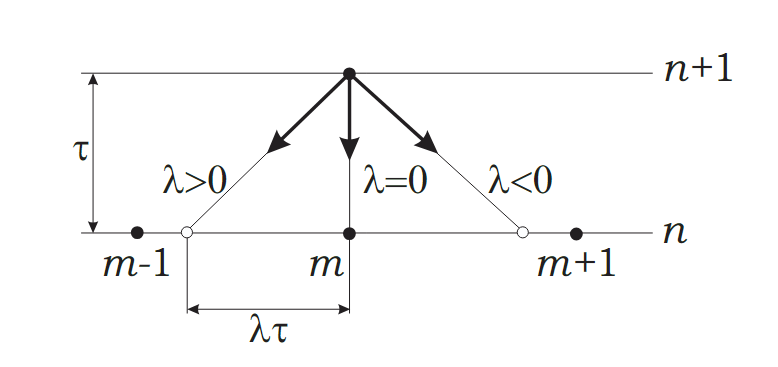
\includegraphics[width=0.7\textwidth]{gcm.png}
	\caption{Иллюстрация сеточно-характеристического метода в одномерном случае}
	\label{fig:gcm}
\end{figure}

Для системы уравнений акустики спектральное разложение выглядит довольно просто и было описано в \cite{kazakov}. Приведем лишь результат разложения. Вдоль направления $\vec{e}$ оно выглядит следующим образом:

\begin{equation}
	\mathbf{A} = \frac{1}{2}
	\begin{pmatrix}
		\vec{e} & \vec{e} & \vec{e'} & \vec{e''} \\
		c\rho & -c\rho & 0 & 0
	\end{pmatrix}
	\begin{pmatrix}
		c & 0 & 0 & 0 \\
		0 & -c & 0 & 0 \\
		0 & 0 & 0 & 0 \\
		0 & 0 & 0 & 0
	\end{pmatrix}
	\begin{pmatrix}
		\vec{e}^T & \dfrac{1}{c\rho} \\
		\vec{e}^T & -\dfrac{1}{c\rho} \\
		2\vec{e'}^T & 0 \\
		2\vec{e''}^T & 0
	\end{pmatrix}
\end{equation}
В данном контексте $\vec{e}$, $\vec{e'}$, $\vec{e''}$ образуют правую тройку, а собственные значения $c$ матрицы $\mathbf{A}$ равны

\begin{equation}
	\begin{aligned}
		c &= \pm \sqrt{\frac{K}{\rho}}, \\
		c &= 0
	\end{aligned}
\end{equation}

\subsection{Программный комплекс}
В настоящей работе используется программный комплекс, реализующий СХМ в 3D на языке Python. Его автором является А. В. Васюков \cite{gcm}. Выбор именно такого комплекса заключается в простоте использования и удобстве доработки, однако пришлось жертвовать скоростью расчетов. Расчеты производятся на ортогональной сетке, примерное время одного расчета --- десятки минут. Простота использования заключается в удобстве понимания и написания программного кода на языке Python, благодаря чему без особых усилий можно варьировать граничные условия и параметры среды. Проще говоря, при таком подходе большее количество сил и времени можно потратить на создание экспериментальной установки, что в настоящей работе оказалось нетривиальной задачей. Визуализация и контроль решения производились в среде ParaView, а также средствами библиотеки matplotlib.

\newpage
